\documentclass[10.5pt,a4paper]{article}
\usepackage{kotex}
\usepackage{fontspec}
\setmainfont{Noto Sans CJK KR}
\setsansfont{Noto Sans CJK KR}
\setmonofont{Noto Sans Mono CJK KR}
\usepackage[a4paper,margin=20mm,headheight=14pt]{geometry}
\usepackage{amsmath,amssymb,mathtools}
\usepackage{booktabs,longtable,tabularx,array,multirow}
\usepackage{enumitem}
\usepackage{tikz}
\usetikzlibrary{arrows.meta,positioning,fit,calc,backgrounds}
\usepackage[most]{tcolorbox}
\usepackage{xcolor}
\usepackage{hyperref}
\usepackage{fancyhdr}
\usepackage{titlesec}
\usepackage{microtype}
\usepackage{graphicx}
\usepackage{caption}
\usepackage{float}
\usepackage{siunitx}
\usepackage{natbib}
\usepackage{setspace}

\definecolor{ink}{HTML}{111111}
\definecolor{accent}{HTML}{274C77}
\definecolor{linegray}{HTML}{C8CDD2}
\definecolor{panel}{HTML}{F5F6F7}
\definecolor{panelblue}{HTML}{EEF3F8}
\color{ink}
\hypersetup{colorlinks=true,linkcolor=accent,citecolor=accent,urlcolor=accent}
\setlength{\parindent}{0pt}
\setlength{\parskip}{0.55em}
\setstretch{1.08}
\setlist[itemize]{leftmargin=1.6em,itemsep=0.2em,topsep=0.25em}
\setlist[enumerate]{leftmargin=1.7em,itemsep=0.25em,topsep=0.25em}
\titleformat{\section}{\Large\bfseries}{\thesection.}{0.55em}{}
\titleformat{\subsection}{\large\bfseries}{\thesubsection.}{0.5em}{}
\titleformat{\subsubsection}{\normalsize\bfseries}{\thesubsubsection.}{0.45em}{}
\titlespacing*{\section}{0pt}{1.2em}{0.45em}
\titlespacing*{\subsection}{0pt}{0.9em}{0.35em}
\pagestyle{fancy}
\fancyhf{}
\lhead{CATENA 연구 실행계획}
\rhead{REALM @ EMNLP 2026}
\cfoot{\thepage}
\renewcommand{\headrulewidth}{0.3pt}

\newcolumntype{Y}{>{\raggedright\arraybackslash}X}
\newcolumntype{L}[1]{>{\raggedright\arraybackslash}p{#1}}
\newtcolorbox{keybox}[1][]{colback=panelblue,colframe=accent,boxrule=0.6pt,arc=2pt,left=8pt,right=8pt,top=6pt,bottom=6pt,#1}
\newtcolorbox{plainbox}[1][]{colback=panel,colframe=linegray,boxrule=0.5pt,arc=2pt,left=8pt,right=8pt,top=6pt,bottom=6pt,#1}
\newcommand{\code}[1]{\texttt{#1}}
\newcommand{\HRule}{\rule{\linewidth}{0.5pt}}

\begin{document}

\begin{titlepage}
\vspace*{15mm}
{\Huge\bfseries CATENA}\par
\vspace{2mm}
{\LARGE Transaction-Conditioned State Transport for Coherent Recurrent Agents}\par
\vspace{8mm}
{\Large\bfseries 4-GPU Full-Access 워크샵 제출 전 연구 실행계획}\par
\vspace{4mm}
{\large REALM @ EMNLP 2026 제출 전 연구계획}\par
\vspace{14mm}
\HRule
\vspace{8mm}
\begin{keybox}
\textbf{중심 질문}\quad 검증된 외부 메모리 트랜잭션이 주어졌을 때, 기존 recurrent execution state를 전체 이력 재실행 없이 짧은 native forward로 갱신하여, 최신 외부 상태에서 다시 구성한 exact-refresh state와 행동적으로 일치시킬 수 있는가?
\end{keybox}
\vspace{8mm}
\begin{tabularx}{\textwidth}{@{}L{34mm}Y@{}}
연산 환경 & NVIDIA RTX PRO 6000 Blackwell Server Edition host 8장 중 GPU 0--3 네 장 할당, full SSH/rootless user-space control, CUDA Toolkit 13.0, NVIDIA driver 580.126.16 \\
주 모델 & RWKV-7 2.9B recurrent LM; Transformer 경계 비교는 Qwen2.5-3B-Instruct \\
제출 목표 & REALM @ EMNLP 2026 archival short 또는 long paper \\
직접 제출 마감 & 2026년 8월 5일 23:59 AoE \\
\end{tabularx}
\vfill
{\small 작성 기준일: 2026년 7월 23일 · 실행 환경 반영 개정본}
\end{titlepage}

\tableofcontents
\newpage

\section{요약: GPU가 늘어도 연구 질문은 바꾸지 않는다}

네 장의 표준 GPU 할당을 SSH로 직접 제어할 수 있게 되면서 바뀐 것은 \textbf{연구의 중심 질문}이 아니라 \textbf{실험의 완결성과 비교의 공정성}이다. 기존의 100만원 예산안에서는 text-only baseline과 단일 transport pilot만으로도 워크샵 제출을 성립시키는 것이 우선이었다. 네 장의 GPU와 full SSH access를 확보한 현재는 다음 약점을 실제 실험으로 보완할 수 있다.

\begin{itemize}
\item RWKV transport encoder를 여러 seed와 slot 수로 학습하여 결과의 우연성을 줄인다.
\item 16K--32K history, 긴 transaction chain, update 이후 긴 query gap을 포함한다.
\item Transformer에 단순 KV append만 주지 않고, learned soft patch와 oracle suffix re-prefill까지 비교한다.
\item 실제 wall-clock latency, state/KV resident bytes, TTFA와 decode 비용을 같은 서버에서 측정한다.
\item exact teacher, 데이터 split, checkpoint, raw prediction과 시스템 로그를 고정하여 재현성을 높인다.
\end{itemize}

이번 제출의 실험 범위는 \textbf{verified transaction이 주어진 뒤 execution state를 어떻게 동기화하는가}에 집중한다. Graph memory, learned writer, branch/merge와 online RL은 워크샵 이후의 확장 경로에서 별도 가설로 연결한다. REALM은 4쪽 또는 8쪽 논문을 받으며, 4쪽 archival short paper에는 작은 집중 기여와 부정적 결과도 허용한다. 따라서 H1--H4 중 확보된 증거의 깊이에 따라 4쪽/8쪽을 결정한다~\citep{realm2026}.

\section{연구 문제와 핵심 개념}

\subsection{외부 상태의 최신성과 내부 실행 상태의 최신성은 다르다}

에이전트의 외부 정규 상태를 $M_t$라 하자. API 규칙, 사용자 권한, workflow 설정처럼 현재 행동의 기준이 되는 사실이 여기에 들어간다. 검증된 트랜잭션 $f_t$가 적용되면
\begin{equation}
M_{t+1}=f_t(M_t)
\end{equation}
가 된다. 그러나 모델이 이미 긴 이력을 처리하여 만든 내부 실행 상태 $S_t$에는 $M_t$에서 유효했던 규칙과 그 규칙으로부터 파생된 계획이 남아 있을 수 있다. 외부 데이터베이스가 최신이라는 사실만으로 $S_t$가 자동 갱신되지는 않는다.

\begin{figure}[H]
\centering
\begin{tikzpicture}[
  font=\small,
  box/.style={draw=linegray,fill=panel,rounded corners=2pt,minimum width=29mm,minimum height=10mm,align=center,inner sep=3pt},
  strong/.style={draw=accent,fill=panelblue,rounded corners=2pt,minimum width=31mm,minimum height=10mm,align=center,inner sep=3pt},
  smallbox/.style={draw=linegray,fill=white,rounded corners=2pt,minimum width=24mm,minimum height=9mm,align=center,inner sep=2.5pt},
  arr/.style={-{Latex[length=2.2mm]},thick,draw=ink}
]
% Exact-refresh reference path
\node[box] (m0) at (0,2.3) {$M_t$\\이전 정규 상태};
\node[box] (m1) at (4.2,2.3) {$M_{t+1}$\\최신 정규 상태};
\node[box] (se) at (8.5,2.3) {$S_{t+1}^{\mathrm{exact}}$\\exact refresh};
\draw[arr] (m0) -- node[above]{검증된 $f_t$} (m1);
\draw[arr] (m1) -- node[above]{전체 재구성} (se);

% CATENA transport path
\node[smallbox] (tx) at (0,0) {$f_t,\operatorname{cl}(f_t)$};
\node[smallbox] (enc) at (3.4,0) {$E_\phi$\\transaction encoder};
\node[smallbox] (z) at (6.5,0) {$Z_t$\\$K$ slots};
\node[box] (native) at (9.6,0) {$F_\theta^{(K)}$\\native forward};
\node[strong] (sc) at (13.0,0) {$S_{t+1}^{\mathrm{CATENA}}$\\transported state};
\node[box] (s0) at (9.6,-1.65) {$S_t$\\기존 실행 상태};
\draw[arr] (tx) -- (enc);
\draw[arr] (enc) -- (z);
\draw[arr] (z) -- (native);
\draw[arr] (s0) -- (native);
\draw[arr] (native) -- (sc);

% Behavioral comparison
\node[smallbox] (cmp) at (13.0,2.3) {미래 질의\\행동 분포 비교};
\draw[arr] (se) -- (cmp);
\draw[arr] (sc) -- (cmp);
\end{tikzpicture}
\caption{위 경로는 전체 재구성으로 만든 operational reference이고, 아래 경로는 기존 실행 상태에 짧은 transaction update만 적용하는 CATENA다. 평가는 hidden vector 자체가 아니라 미래 행동의 일치도로 수행한다.}
\end{figure}

\subsection{용어와 변수}

\begin{longtable}{@{}L{33mm}L{45mm}p{82mm}@{}}
\toprule
기호/용어 & 이름 & 정의 \\
\midrule
\endhead
$t$ & 논리적 상태 버전 & 다음 token 번호가 아니라 transaction commit 전후를 구분하는 인덱스다. \\
$M_t$ & canonical external state & 현재 행동의 기준이 되는 versioned 외부 상태다. \\
$S_t$ & execution state & 모델이 현재 목표, 최근 관찰, 이전 계획을 압축해 보유하는 내부 계산 상태다. RWKV에서는 고정 크기 recurrent state다. \\
$f_t$ & verified transaction & schema와 precondition 검증을 통과해 $M_t$를 $M_{t+1}$로 바꾸는 연산이다. \\
$\operatorname{cl}(f_t)$ & dependency closure & 직접 바뀐 항목과 그 항목에 의존하여 재계산 또는 무효화가 필요한 항목 집합이다. \\
$E_\phi$ & transaction encoder & $f_t$와 closure를 $K$개의 연속 입력 slot으로 압축하는 작은 학습 모듈이다. \\
$Z_t$ & transaction slots & $Z_t=E_\phi(f_t,\operatorname{cl}(f_t))\in\mathbb{R}^{K\times d}$다. query는 encoder 입력에 넣지 않는다. \\
$F_\theta$ & native forward & frozen backbone의 원래 recurrent transition이다. hidden tensor에 임의 delta를 더하지 않는다. \\
$S_{t+1}^{\mathrm{exact}}$ & operational reference & 이전 사건을 지우지 않고, 검증된 update와 최신 canonical view를 포함한 refresh input을 처음부터 처리해 얻는 기준 상태다. 유일한 ``정답 벡터''가 아니라 동일 backbone의 reference다. \\
$S_{t+1}^{\mathrm{CATENA}}$ & transported state & 기존 $S_t$에서 $K$개의 slot만 native forward로 처리해 만든 실제 배포 상태다. \\
state transport & 상태 이동 & $M_t\to M_{t+1}$의 변경에 맞춰 $S_t$를 새 외부 상태와 양립하는 실행 상태로 보내는 연산이다. \\
behavioral coherence & 행동적 일관성 & 두 hidden state의 좌표가 같은지가 아니라, 여러 미래 질의와 도구 행동에서 exact reference와 같은 결정을 내리는지다. \\
\bottomrule
\end{longtable}

CATENA의 transport는 다음과 같이 정의한다.
\begin{align}
Z_t &= E_\phi\!\left(f_t,\operatorname{cl}(f_t)\right),\\
S_{t+1}^{\mathrm{CATENA}} &= T_{\phi,f_t}(S_t)=F_\theta^{(K)}(S_t,Z_t).
\end{align}
Exact reference는 과거를 새 사실로 덮어쓰는 것이 아니라, 이전 사건을 보존한 채 transaction과 최신 canonical view를 반영한 refresh input $H_{t+1}^{\mathrm{refresh}}$로부터 얻는다.
\begin{equation}
S_{t+1}^{\mathrm{exact}}=R_\theta\!\left(H_{t+1}^{\mathrm{refresh}}\right).
\end{equation}
목표는 $S_{t+1}^{\mathrm{CATENA}}=S_{t+1}^{\mathrm{exact}}$라는 벡터 동일성이 아니다. 미래 행동 분포가 가까워지는 것이다.
\begin{equation}
p_\theta(y\mid S_{t+1}^{\mathrm{CATENA}},q)\approx p_\theta(y\mid S_{t+1}^{\mathrm{exact}},q).
\end{equation}

\subsection{성공은 correction과 retention을 동시에 요구한다}

변경의 영향을 받는 질의 집합을 $Q_{\mathrm{aff}}$, 영향을 받지 않는 작업 문맥을 묻는 질의 집합을 $Q_{\mathrm{keep}}$라 한다. 정책 $\pi$의 correction과 retention은 다음과 같다.
\begin{align}
C_{\mathrm{update}}(\pi)&=\Pr[\hat y^\pi=\hat y^{\mathrm{exact}}\mid q\in Q_{\mathrm{aff}}],\\
C_{\mathrm{retain}}(\pi)&=\Pr[\hat y^\pi=\hat y^{\mathrm{exact}}\mid q\in Q_{\mathrm{keep}}],\\
C_{\mathrm{joint}}(\pi)&=\frac{2C_{\mathrm{update}}C_{\mathrm{retain}}}{C_{\mathrm{update}}+C_{\mathrm{retain}}}.
\end{align}
새 규칙만 반영하고 기존 사용자 선택을 잊으면 destructive overwrite다. 반대로 문맥은 보존하지만 새 규칙을 반영하지 못하면 stale state다. CATENA는 joint coherence와 갱신 비용을 함께 개선해야 한다.

\section{왜 RWKV인가: 우월성 주장이 아니라 실험적 기질의 선택}

RWKV-7은 history 길이에 따라 커지는 KV cache 대신 명시적인 fixed-size recurrent state를 노출하고, token 또는 embedding 입력을 같은 state transition으로 처리할 수 있어 transaction-conditioned state transport 가설을 비교적 낮은 구현 복잡도로 격리하기 좋다~\citep{rwkv7}. 본 연구에서 RWKV는 Transformer나 Mamba보다 본질적으로 우월하다는 전제가 아니라, \textbf{고정 차원 실행 상태 위에서 transport를 정의하고 비용을 측정하기 위한 실험용 기반}이다.

메인 결과는 differentiable FLA/HF model인 \code{fla-hub/rwkv7-2.9B-g1}으로 고정한다. 이 model card가 가리키는 원본은 \code{rwkv7-g1-2.9b-20250519-ctx4096.pth}이므로, 공식 PTH runtime 교차 검증도 반드시 같은 source weight를 사용한다~\citep{rwkvmodel}. 최신 PTH와 과거 FLA conversion을 한 결과표에 섞지 않는다. 더 최신 checkpoint의 transfer 결과는 main claim이 고정된 뒤의 보조 분석으로만 다룬다. Transformer 경계 비교는 parameter 규모와 context 지원이 가까우며 HF runtime이 안정적인 Qwen2.5-3B-Instruct를 사용한다~\citep{qwen25model,qwen25report}.

\section{연산 환경과 4-GPU 운용 원칙}

2026년 7월 25일 E00 audit에서 host는 NVIDIA RTX PRO 6000 Blackwell Server Edition 8장을 노출했으며, 표준 4-lane 할당은 같은 NUMA 권역의 물리 GPU 0--3으로 고정했다. 선택된 각 GPU는 97,887 MiB, compute capability 12.0, MIG Disabled였고 driver 580.126.16과 CUDA Toolkit 13.0을 확인했다. CUDA 문서상 13.x minor-version compatibility는 driver branch 580 이상을 요구하며, 580.126.16은 이 범위에 속한다~\citep{rtxpro6000,cuda13compat}. Conda \code{catena}에는 공식 CUDA 13.0 wheel인 PyTorch 2.12.1+cu130과 선언된 Python package를 고정했다~\citep{pytorch212}. GPU 0--3은 native \code{sm\_120} BF16-input cuBLAS GEMM과 PyTorch BF16 matmul에서 모두 finite, max absolute error 0을 냈고, UUID/PCI identity, storage integrity와 repository gate까지 포함한 E00 전체가 PASS했다. 따라서 E01 인프라 선행조건은 열렸지만, 이는 H1--H4의 증거가 아니므로 과학적 가설과 평가 설계는 바꾸지 않는다.

\subsection{소프트웨어 stack}

\begin{tabularx}{\textwidth}{@{}L{38mm}Y@{}}
\toprule
항목 & 고정안 \\
\midrule
운영 & full SSH, \code{tmux} persistent sessions, local model cache, process-level GPU binding \\
Python & 3.11 \\
PyTorch & 2.12.1+cu130 wheel (system toolkit과 분리하여 pin) \\
정밀도 & BF16 기본; metric accumulation은 FP32 \\
Transformer & Hugging Face Transformers 5.14.1 (E00 snapshot; E01 compatibility gate) \\
RWKV & 동일 source weight의 FLA/HF differentiable path를 main으로 사용; 공식 PTH path는 inference 교차 검증 \\
로그 & config snapshot, git SHA, host audit, seed, raw prediction, latency samples, checkpoint hash \\
\bottomrule
\end{tabularx}

\subsection{네 장은 분산학습보다 네 개의 독립 실험 lane으로 사용한다}

3B backbone은 한 장의 96GB급 GPU에 충분히 적재될 가능성이 높고, 이 연구의 병목은 하나의 대규모 최적화가 아니라 teacher 생성, seed, ablation과 architecture boundary의 수다. 따라서 기본값은 DDP/tensor parallel이 아니라 GPU별 독립 process다. P2P/NVLink 여부는 기록하되 core experiment의 전제에 두지 않는다.

\begin{table}[H]
\centering
\begin{tabularx}{\textwidth}{@{}L{22mm}L{44mm}Y@{}}
\toprule
단계 & GPU 0--2 & GPU 3 \\
\midrule
E00--E02 & 동일 environment/runtime/data gate를 GPU별 반복 & Qwen 및 cache crop hard gate \\
E03--E04 & RWKV test shard 0--2 & RWKV test shard 3 또는 Qwen text pilot \\
E05 & RWKV exact-teacher shard 0--2 & exact-teacher shard 3 \\
E06 & typed $K=4,8,16$ slot sweep & parameter-matched generic slot \\
E07 & 선택된 $K$의 seeds 11/22/33 & no-closure/untyped ablation \\
E08 & Qwen boundary shard 또는 learned patch seeds & profiling/remaining boundary run \\
E09 & H4 composition seeds 11/22/33 & matched distillation-only seeds 11/22/33 \\
E10--E12 & final profiling, test shards, clean rerun & figure generation 및 재현 검증 \\
\bottomrule
\end{tabularx}
\end{table}

네 장을 13일 동안 100\% 점유하면 이론상 약 1,248 GPU-hour지만, adapter 디버깅, 데이터 검증과 원고 작성 시간을 고려한 현실적인 목표는 800--1,050 GPU-hour다. full access의 실질적 이점은 local model cache, custom-kernel compile, persistent \code{tmux}, 장시간 profiling과 네 개의 독립 job을 동시에 운용할 수 있다는 점이다. Transformer full KV는 디스크에 저장하지 않고 token boundary와 teacher logits만 보존한다.

\section{공통 데이터: CATENA-UpdateBench}

\subsection{episode 구조}

각 episode는 다음 요소를 가진다.

\begin{enumerate}
\item 변경 전 canonical state $M_t$와 그 규칙으로 형성된 execution history.
\item old rule을 사용한 derived plan 또는 tool action.
\item verified transaction $f_t$와 dependency closure.
\item 변경 후 canonical state $M_{t+1}$.
\item 영향을 받는 direct query, 파생 tool-call query, 영향을 받지 않는 retention query.
\item exact refresh를 위한 operational reference input과 Transformer suffix boundary.
\end{enumerate}

도메인은 API configuration, access-control policy, user/workflow state 세 개로 고정한다. 메인 변수는 history length, dependency depth, operation type, query gap, transaction chain length, schema/template split이다.

\begin{table}[H]
\centering
\begin{tabularx}{\textwidth}{@{}L{37mm}Y@{}}
\toprule
변수 & 값과 목적 \\
\midrule
History length & 1K, 4K, 8K, 16K; 32K stress. history scaling과 KV resident cost 측정 \\
Query kind & affected-direct, affected-derived/tool, unaffected-retention \\
Operation & SUPERSEDE, AMEND 중심; 안정 후 INVALIDATE, ADD\_EXCEPTION \\
Dependency depth & 0, 1, 2. closure 필요성을 분리 \\
Update-to-query gap & 0, 128, 512, 2,048 token. stale resurfacing과 지속성 평가 \\
Chain length & train 1--2, test 4/8/16 \\
OOD split & unseen wording, entity schema, operator pair, path \\
\bottomrule
\end{tabularx}
\end{table}

학습용 후보 규모는 6K--12K episode, validation 1K 내외, test 2K--4K를 목표로 하되, 실제 tokenization 속도와 teacher 비용을 Day 2에 측정하여 고정한다. 모든 split과 generator version은 제출 전에 freeze한다.

\section{실험 프로그램 전체 지도}

실험은 H1--H4를 단순히 나열하지 않고, 앞 단계가 다음 단계의 필요조건을 제공하도록 순서화한다. E00--E02는 측정 도구와 데이터의 타당성을 고정하고, E03--E04는 학습 없이 문제와 update signal을 검증한다. E05 이후에만 learned transport를 학습하며, H3가 성립한 뒤 H4를 수행한다.

\begin{longtable}{@{}L{15mm}L{31mm}L{39mm}p{76mm}@{}}
\toprule
단계 & 질문 & 모델/학습 & 핵심 산출물과 gate \\
\midrule
\endhead
E00 & 서버가 재현 가능한가 & 모델 없음 & GPU/VRAM/topology, CUDA/PyTorch, storage와 compiler manifest \\
E01 & adapter가 올바른가 & RWKV 0.4B/2.9B, Qwen 3B; 학습 없음 & token--embedding, chunk, clone, crop, gradient parity \\
E02 & 데이터가 누출 없이 문제를 격리하는가 & generator/validator & fixed pilot/main/stress/chain split과 hash \\
E03/H1 & stale state가 실제 오류를 만드는가 & RWKV 2.9B; 학습 없음 & stale--exact paired gap, teacher ceiling \\
E04/H2 & 어떤 transaction 표현이 필요한가 & RWKV 2.9B; 학습 없음 & plain/typed/closure/reset/retrieval/Tx-only ablation \\
E05 & exact reference를 재사용할 수 있는가 & RWKV exact forward & train/val candidate-distribution teacher cache \\
E06 & transport가 학습되며 $K$는 얼마인가 & frozen RWKV + slot encoder & 300-step gate, $K=4/8/16$ one-seed sweep \\
E07/H3 & compact transport가 Pareto를 개선하는가 & 선택 $K$, 3 seeds + ablations & main/stress coherence--cost result \\
E08 & Transformer에서 어느 repair가 필요한가 & Qwen, inference + learned soft patch & append/capsule/suffix/full re-prefill regime map \\
E09/H4 & composition이 긴 chain drift를 줄이는가 & H3 init, chain 1--2 학습 & test 4/8/16 drift vs matched control \\
E10 & 실제 비용은 무엇인가 & 두 backbone & p50/p95 latency, TTFA, decode, state/KV bytes \\
E11 & 실제 tool action으로 이어지는가 & 자연화 subset 생성 평가 & JSON validity, argument match, simulator success \\
E12 & 어떤 claim이 재현되는가 & 선택된 config clean rerun & raw predictions, figures, anonymous package \\
\bottomrule
\end{longtable}

\section{시간 순서별 실험 계획}

\subsection{E00--E02. 환경, runtime, 데이터 hard gate}

\textbf{인사이트.} H3의 효과보다 먼저 확인할 것은 모델 adapter가 올바른가다. token ID 경로와 embedding 경로가 다르면 transport 개선 또는 실패를 해석할 수 없다.

\textbf{실행.}
\begin{itemize}
\item \code{nvidia-smi}, topology, CUDA/PyTorch, BF16, storage audit.
\item RWKV full sequence 대 chunked sequence의 logits/state 일치.
\item token ID 입력 대 동일 token embedding 직접 입력의 logits 일치.
\item state clone 간 alias 부재, serialize/restore 후 candidate logits 일치.
\item Qwen KV cache truncate/reuse와 full prefill의 prefix logits 일치.
\end{itemize}

\textbf{통과 기준.} inference-only 경로와 differentiable embedding 경로의 candidate ranking이 동일하고, numerical error가 BF16 tolerance 안에 있어야 한다. custom CUDA extension이 실제 Blackwell compute capability를 지원하지 않으면 E1/H2는 text runtime으로 진행하되 H3 시작 전 adapter를 수정한다.

\subsection{E03/H1. 외부 상태만 바꾸면 stale execution-state failure가 발생하는가}

\begin{keybox}
\textbf{H1.} $M_t\to M_{t+1}$ 이후 $S_t$를 그대로 재사용하면, exact refresh보다 폐기된 행동을 선택하는 비율이 높아진다.
\end{keybox}

\textbf{데이터와 모델.} RWKV-7 2.9B, 3개 도메인의 test episode, history 1K/4K/8K/16K. 학습은 하지 않는다.

\textbf{비교.}
\begin{enumerate}
\item \textbf{Stale reuse}: $S_t$를 그대로 사용.
\item \textbf{Exact refresh}: transaction과 최신 canonical view를 포함한 전체 reference input으로 $S_{t+1}^{\mathrm{exact}}$를 재구성.
\end{enumerate}

\textbf{메트릭.} Gold accuracy, own-oracle agreement, teacher-correct agreement, stale-action rate, $C_{\mathrm{update}}$, $C_{\mathrm{retain}}$, $C_{\mathrm{joint}}$, behavioral KL.

\textbf{검증 결과.} Exact teacher가 gold task를 충분히 풀며, stale reuse가 affected query에서 paired bootstrap CI 기준으로 유의하게 낮아야 H1이 지지된다. retention query는 두 조건에서 비슷해야 한다. exact 자체가 약하면 task/backbone ceiling 문제이며, stale-exact gap이 없으면 benchmark가 coherence failure를 유도하지 못한 것이다.

\textbf{허용 주장.} H1만 성립하면 ``persistent recurrent state에서 외부 state update 후 functional incoherence가 발생한다''는 진단 결과까지만 주장한다.

\subsection{E04/H2. 어떤 update signal이 필요하며 정답 누출은 아닌가}

\begin{keybox}
\textbf{H2.} operation, version, validity와 dependency closure를 포함한 typed transaction은 plain correction보다 correction을 높이고 retention을 유지하며, 그 이득은 transaction만으로 정답을 직접 제공한 결과가 아니다.
\end{keybox}

\textbf{비교 정책.}
\begin{itemize}
\item Plain correction: ``새 값은 X''.
\item Typed transaction: operation/target/old/new/version.
\item Typed + dependency closure.
\item Shuffled closure: closure 크기는 같지만 관련 key를 섞은 통제.
\item Transaction-only: $S_t$를 제거하고 empty state에서 transaction만 처리하는 누출 통제.
\item Reset + compact canonical snapshot.
\item Query-time latest-memory retrieval.
\item Exact refresh.
\end{itemize}

\textbf{학습.} 없음. 동일 transaction 이후 여러 future query를 사용하며 encoder나 patch 생성에는 query를 넣지 않는다.

\textbf{메트릭.} H1 메트릭에 patch token 수, update latency, correction-retention Pareto를 추가한다.

\textbf{검증 결과.} Closure가 plain/typed보다 affected-derived query를 개선하되 retention을 낮추지 않아야 한다. Transaction-only가 closure와 같은 성능을 내면 기존 state를 이용한 것이 아니며, shuffled closure가 동일하면 dependency 구조의 기여가 없다. Reset 또는 retrieval이 같은 정확도와 비용을 내면 learned transport의 실용적 필요성이 약해진다.

\textbf{허용 주장.} H1+H2가 성립하면 verified typed transaction/closure가 recurrent execution state의 update signal로 유효하다고 주장할 수 있다. 아직 continuous state transport의 우위는 주장하지 않는다.

\subsection{E05. Exact teacher와 실행 manifest 고정}

H3에서 exact refresh와 candidate scoring을 매 step 다시 계산하면 teacher 비용이 학습을 지배한다. E1/H2가 통과하면 train/validation episode에 대해 exact candidate log-likelihood, exact prediction, gold index, token length와 generator/model manifest를 materialize한다.

기본 baseline은 cache object의 backend별 serialization 불확실성을 피하기 위해 teacher logits만 필수 저장한다. H3 trainer는 base history를 다시 prefill하며, E01에서 RWKV fixed state의 CPU serialization/restore가 안정적으로 통과한 경우에만 optional base-state cache를 켠다. Qwen full KV는 저장하지 않고 text와 affected-prefix token boundary만 보존한다. Teacher가 틀린 sample은 제거하지 않고 flag를 남겨 전체와 teacher-correct subset을 함께 보고한다.

\subsection{E06--E07/H3. Compact native state transport}

\begin{keybox}
\textbf{H3.} Query-independent transaction slots를 native recurrent forward에 투입하면, typed text patch보다 짧은 update로 exact-refresh behavior를 근사하고 reset/retrieval/generic soft-slot보다 나은 정확도--비용 Pareto를 만들 수 있다.
\end{keybox}

\textbf{모델.} Frozen RWKV-7 2.9B와 약 5--20M parameter의 TransactionSlotEncoder. 계산을 full factorial로 쓰지 않고 두 단계로 진행한다. 먼저 seed 11에서 $K\in\{4,8,16\}$과 generic $K=8$을 비교해 validation $C_{\mathrm{joint}}$로 $K$를 선택한다. 이후 선택된 $K$에서 seeds 11/22/33을 재학습하고, no-closure, untyped, generic ablation을 제한된 seed로 수행한다.

\textbf{입력.} Typed transaction과 closure의 token embedding. Encoder는 이를 $K$개 slot $Z_t$로 압축한다. query를 입력하지 않고, 한 번 생성한 $S_{t+1}^{\mathrm{CATENA}}$에서 direct, derived, retention query를 모두 평가한다.

\textbf{학습 gate.} 모든 run은 먼저 300 step만 실행하여 finite loss/gradient, validation KL 감소와 exact-teacher ceiling을 확인한다. 통과한 config만 2K--6K step으로 확장한다. Test split은 model/slot 선택에 사용하지 않는다.

\textbf{학습 loss.} Affected query와 retention query를 분리해 exact-refresh teacher의 후보 분포를 증류한다.
\begin{equation}
\mathcal L_{\mathrm{H3}}
=1.0\,D_{\mathrm{KL}}(p_{\mathrm{exact}}^{\mathrm{aff}}\Vert p_{\mathrm{CATENA}}^{\mathrm{aff}})
+0.6\,D_{\mathrm{KL}}(p_{\mathrm{exact}}^{\mathrm{keep}}\Vert p_{\mathrm{CATENA}}^{\mathrm{keep}})
+0.5\,\mathcal L_{\mathrm{gold}}.
\end{equation}
$\mathcal L_{\mathrm{gold}}$는 affected와 retention 후보에 대한 cross-entropy의 평균이다. Backbone parameter는 optimizer에 넣지 않고 transaction encoder만 학습한다. Slot norm penalty는 별도 ablation이 필요하므로 기본 objective에 넣지 않는다.

\textbf{Baseline.}
\begin{itemize}
\item Closure text patch, reset+snapshot, query retrieval, exact refresh.
\item Parameter-matched GenericSoftSlot: 동일 encoder 크기, field name과 typed structure를 제거한 입력.
\item Typed no-closure encoder.
\item Direct hidden delta는 off-manifold negative control로 작은 subset에서만 수행.
\end{itemize}

\textbf{메트릭.} Gold, own-oracle, teacher-correct agreement, correction, retention, joint coherence, behavioral KL, update latency, state bytes, coherence per millisecond. Latency는 warm-up 후 여러 번 측정하고 p50/p95를 보고한다.

\textbf{검증 결과.} CATENA가 text와 generic slot보다 joint coherence 또는 같은 coherence에서 latency를 개선하여 Pareto frontier를 확장해야 한다. Tx-only와 CATENA가 같으면 state transport 주장은 성립하지 않는다. GenericSoftSlot과 같으면 typed 구조의 추가 기여를 주장하지 않는다. Reset/retrieval과 같은 비용--정확도면 transport의 실용적 필요성을 주장하지 않는다.

\textbf{허용 주장.} H1--H3가 모두 지지될 때 ``verified transaction을 compact native inputs로 변환해 recurrent execution state를 exact-refresh behavior에 가깝게 이동시킬 수 있다''고 주장한다.

\subsection{E09/H4. 반복 업데이트와 합성 일반화}

\begin{keybox}
\textbf{H4.} 짧은 transaction chain에서 sequential path와 composed path의 행동을 정렬하면, 같은 chain data를 사용한 distillation-only control보다 길이 4/8/16에서 coherence drift가 작다.
\end{keybox}

학습은 chain length 1--2를 사용한다. 동일 initial state에서 $f$ 후 $g$를 순차 적용한 state와, symbolic engine이 안전하게 합성할 수 있는 macro transaction $g\circ f$를 적용한 state를 비교한다.
\begin{equation}
\mathcal L_{\mathrm{H4}}=
\mathcal L_{\mathrm{exact}}+
\lambda_{\mathrm{path}}D_{\mathrm{KL}}\!\left(p_{T_g(T_f(S))}\Vert p_{T_{g\circ f}(S)}\right).
\end{equation}

\textbf{비교.} Distillation-only matched control과 composition+path consistency를 비교한다. 두 조건은 같은 chain episode와 step 수를 사용하고, 차이는 path-consistency weight뿐이다. 첫 제출에서는 same-key version chain을 중심으로 하고 independent-key commutation은 시간이 남을 때 확장한다.

\textbf{평가.} Chain 4/8/16, query gap 0/128/512/2,048, old-rule resurfacing prompt, unseen operator pair와 schema. Final joint coherence, cumulative KL, drift slope, retention decay, stale recurrence를 측정한다.

\textbf{검증 결과.} Composition/path 조건이 matched distillation-only control보다 긴 chain에서 drift slope를 낮춰야 한다. 차이가 없으면 categorical/compositional novelty를 주장하지 않고 H3 single-update 결과로 논문을 제한한다.

\section{Transformer 경계 실험: KV append만 비교하지 않는다}

Transformer 비교는 메인 토픽을 대체하지 않는다. 목적은 CATENA가 필요한 workload regime과 fixed-size recurrent state의 경계를 확인하는 것이다. Qwen2.5-3B-Instruct를 사용하고 각 모델을 자기 exact oracle에 대해 정규화한다. Raw accuracy와 own-oracle agreement를 함께 보고한다.

\begin{table}[H]
\centering
\begin{tabularx}{\textwidth}{@{}L{42mm}Y@{}}
\toprule
Transformer 정책 & 의미 \\
\midrule
Stale KV reuse & 외부 state만 바뀌고 기존 token-indexed cache를 그대로 사용 \\
Plain/typed/closure append & 기존 KV 뒤에 정정 정보를 정상 forward로 추가 \\
Learned soft patch & H3와 parameter/slot 수를 맞춘 continuous input patch; fairness check \\
Reset + compact capsule & KV를 버리고 현재 canonical state와 작업 요약만 재입력 \\
Oracle affected-suffix re-prefill & 영향받은 최초 위치 이전 prefix KV는 재사용하고, 그 이후 current-view suffix만 정확히 재계산 \\
Full re-prefill & 전체 reference input을 다시 처리하는 exact oracle \\
\bottomrule
\end{tabularx}
\end{table}

특정 위치의 K/V tensor만 overwrite하는 방법은 메인 baseline으로 두지 않는다. 이후 token들의 KV에 이전 사실에서 파생된 표현이 남을 수 있기 때문이다. 필요하면 작은 negative-control subset에서만 수행한다. Transformer learned patch도 3 seed를 기본으로 두어 RWKV H3와 같은 데이터, slot 수, encoder 규모와 loss로 비교한다.

\textbf{측정.} Own-oracle correction/retention/joint, gold accuracy, patch 또는 re-prefill latency, TTFA, 이후 32-token decode latency, resident KV bytes, history length와 update frequency에 따른 scaling.

\textbf{해석.} 결과는 ``RWKV가 항상 우수하다''가 아니라 다음 regime map으로 제시한다.
\begin{itemize}
\item 긴 active history와 빈번한 state update에서 fixed recurrent state가 유리한가.
\item exact string recall, distributed cross-reference와 희소 update에서는 KV cache가 유리한가.
\item Append correction이 충분한 조건과 suffix/full repair가 필요한 조건은 무엇인가.
\end{itemize}
Transformer가 전 조건에서 더 정확하고 비용도 낮으면 recurrent-specific advantage는 주장하지 않는다. 이 경우 architecture boundary 분석은 남지만 H3의 실용적 범위는 좁아진다.

\section{4-GPU 실행 일정: 2026-07-23부터 2026-08-05까지}

7월 25일 현재 E00 dependency gate는 PASS하여 E01의 인프라 선행조건이 열렸다. 과학적 실험 순서와 gate는 아래 원안대로 유지한다. 다만 이미 지난 7월 24--25일 E01--E03 달력은 저장공간 확보와 E01 완료 시점부터 다시 배치해야 한다. 모델, teacher cache와 checkpoint를 만들기 전에 repository-local 여유 공간 약 25 GiB를 권장 128 GiB 이상으로 확보하거나 저장소 내부의 대체 위치를 정한다. GPU 4--7은 별도 계획 변경 없이 seed나 결과 수를 늘리는 데 사용하지 않는다. FLA 설치 등 package snapshot 변경 뒤에는 E00을 다시 PASS한다.

\begin{longtable}{@{}L{22mm}L{43mm}p{92mm}@{}}
\toprule
날짜 & 주 작업 & 완료 조건 \\
\midrule
\endhead
7/23 & E00 환경 audit와 repo smoke & 4 GPU/VRAM/topology, PyTorch cu130, BF16, storage와 compiler manifest \\
7/24 & E01 RWKV/Qwen backend gate & RWKV token--embedding/chunk/clone/gradient, Qwen crop/suffix parity \\
7/25 & E02 pilot data와 E03/H1 gate & exact teacher ceiling, stale gap, leakage audit; H1 Go/No-Go \\
7/26 & E04/H2 full representation ablation & plain/typed/closure/Tx-only/reset/retrieval 결과 \\
7/27 & Main split freeze와 E05 teacher shards & dataset hash, RWKV train/val teacher cache \\
7/28 & E06 300-step pilot와 $K=4/8/16$ sweep & finite gradient, validation 기준 selected $K$ \\
7/29--30 & E07 H3 three seeds와 ablation & main checkpoint, generic/no-closure/untyped controls \\
7/30--31 & E08 Qwen inference boundary와 teacher & append/capsule/suffix/full results, learned-patch teacher \\
7/31--8/1 & Transformer learned patch와 E09/H4 & 3-seed fairness, H4 composition 3 seeds vs matched control 3 seeds \\
8/1 & paper claim/length gate & H1--H3 강하면 8쪽, 아니면 4쪽 focused/negative result \\
8/2 & E10/E11 final test와 profiling & Pareto, drift, regime map, tool-call subset freeze \\
8/3 & 통계/그림/본문 통합 & paired bootstrap, claim matrix와 table 일치 \\
8/4 & E12 clean rerun와 anonymous package & clean command, PDF preflight, config/model/data hash \\
8/5 & 최종 제출 & OpenReview 23:59 AoE 이전 업로드 \\
\bottomrule
\end{longtable}

실험과 원고를 직렬화하지 않는다. Day 2부터 Introduction, Method와 Benchmark 정의는 고정하고, validation 결과로 고른 config만 test에 적용한다. REALM 공식 공지의 직접 제출 마감과 4/8쪽 형식을 기준으로 한다~\citep{realm2026}.

\section{Repository 구조와 실험 산출물}

저장소는 모델별이 아니라 실험 단계별로 찾을 수 있게 구성한다. 배포 기준 baseline은 이 문서와 함께 제공하는 \code{v0.6.0} 저장소다.

\begin{figure}[H]
\centering
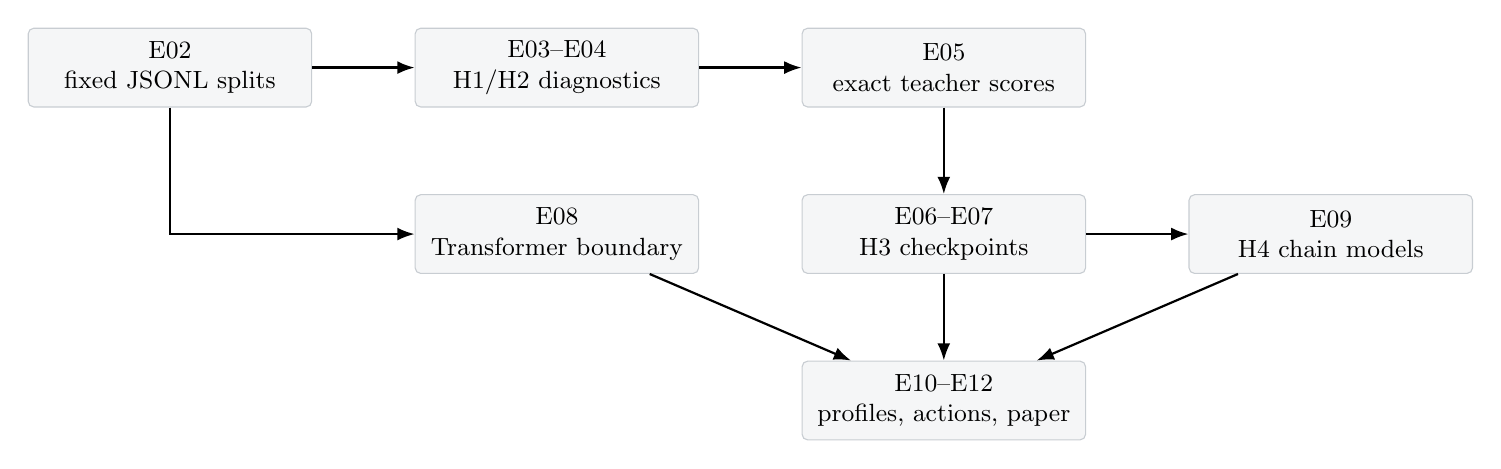
\begin{tikzpicture}[
  font=\small,
  node distance=11mm and 13mm,
  box/.style={draw=linegray,fill=panel,rounded corners=2pt,minimum width=36mm,minimum height=10mm,align=center},
  arr/.style={-{Latex[length=2.2mm]},thick}
]
\node[box] (data) {E02\\fixed JSONL splits};
\node[box, right=of data] (diag) {E03--E04\\H1/H2 diagnostics};
\node[box, right=of diag] (teacher) {E05\\exact teacher scores};
\node[box, below=of teacher] (h3) {E06--E07\\H3 checkpoints};
\node[box, left=of h3] (tr) {E08\\Transformer boundary};
\node[box, right=of h3] (h4) {E09\\H4 chain models};
\node[box, below=of h3] (final) {E10--E12\\profiles, actions, paper};
\draw[arr] (data) -- (diag);
\draw[arr] (diag) -- (teacher);
\draw[arr] (teacher) -- (h3);
\draw[arr] (data) |- (tr);
\draw[arr] (h3) -- (h4);
\draw[arr] (tr) -- (final);
\draw[arr] (h3) -- (final);
\draw[arr] (h4) -- (final);
\end{tikzpicture}
\caption{저장소 산출물은 E02 데이터에서 시작해 진단, teacher, H3/H4와 Transformer boundary를 거쳐 최종 표와 원고로 수렴한다.}
\end{figure}

\begin{tabularx}{\textwidth}{@{}L{47mm}Y@{}}
\toprule
경로 & 역할 \\
\midrule
\code{configs/data/} & E02 smoke/pilot/main/stress/chain split 생성 설정 \\
\code{configs/models/} & 동일 source RWKV FLA/PTH와 Qwen 설정 \\
\code{configs/experiments/} & E00--E11의 실행 단위, seed, loss와 출력 경로 \\
\code{src/catena/data/} & episode/chain generator, schema, rendering과 validator \\
\code{src/catena/methods/} & text update policy, encoder input와 transaction slot encoder \\
\code{src/catena/models/} & recurrent state와 Transformer KV cache의 공통 adapter \\
\code{src/catena/training/} & exact teacher, H3/H4 trainer와 loss \\
\code{src/catena/experiments/} & inference/H3/H4 evaluation, profiling과 tool-call runner \\
\code{src/catena/eval/} & coherence metric, bootstrap와 shard merge \\
\code{scripts/} & 기존 Conda \code{catena}의 CUDA 13 audit, config/runtime gate, E03--E12 4-GPU entry point \\
\code{docs/} & START HERE, runbook, backend gate와 claim ceiling \\
\bottomrule
\end{tabularx}

각 run에는 config snapshot, git SHA, host audit hash, model checkpoint hash, seed, raw prediction JSONL, summary JSON, latency sample을 함께 저장한다. 테스트를 열기 전에 generator와 split hash를 고정하며, tuning은 validation에서만 수행한다.

\section{결과별 허용 주장과 조기 판정}

\begin{longtable}{@{}L{54mm}p{105mm}@{}}
\toprule
관측 결과 & 허용되는 가장 강한 해석 \\
\midrule
\endhead
Exact teacher가 gold를 못 품 & task/backbone ceiling 분석. Transport 효과를 결론 내리지 않음 \\
Stale와 exact 차이가 없음 & 이 설정에서 coherence failure가 유도되지 않았다는 부정 결과 \\
H1만 성립 & persistent execution state의 stale-state failure 진단 \\
H1+H2 성립 & typed transaction/closure가 update signal로 유효 \\
Tx-only $\approx$ CATENA & 기존 state를 실제로 이용한 transport라는 주장은 불가 \\
Reset/retrieval $\approx$ CATENA & learned transport의 실용적 필요성 주장은 불가 \\
GenericSoftSlot $\approx$ typed CATENA & typed structure의 추가 기여는 불가 \\
H1--H3 성립 & compact native state transport와 accuracy--cost Pareto 개선 \\
H4가 matched distillation-only control보다 우수 & compositional regularization의 long-chain 일반화 \\
Transformer repair가 전 범위 우세 & recurrent advantage를 철회하고 boundary analysis로 제한 \\
RWKV가 긴 history/high-update에서만 우세 & 해당 workload regime에 한정한 fixed-state 이점 \\
\bottomrule
\end{longtable}

\section{최종 산출물}

\begin{enumerate}
\item REALM @ EMNLP 2026 4쪽 또는 8쪽 anonymous paper와 appendix.
\item CATENA-UpdateBench generator, fixed train/validation/test/stress split과 hash.
\item H1/H2 text baseline prediction manifest.
\item RWKV TransactionSlotEncoder checkpoint 3 seed와 generic baseline.
\item H4 composition checkpoint 및 long-chain drift 결과.
\item Qwen text/learned/suffix/full re-prefill boundary 결과.
\item 재현 가능한 baseline repository: 기존 Conda 환경 audit, host/CUDA manifest, config, runner, tests, runbook.
\item 논문용 핵심 그림: stale gap, representation ablation, CATENA Pareto, chain drift, architecture regime map.
\end{enumerate}

\section{워크샵 이후의 진화 경로}

워크샵 결과가 state synchronization의 필요성과 compact transport의 가능성을 보이면, 다음 단계에서 다음을 결합한다.

\begin{itemize}
\item Risk-calibrated selective exact refresh: transport 실패 확률이 높은 update만 exact replay.
\item Bitemporal canonical memory와 learned transaction writer: raw observation에서 verified transaction까지 확장.
\item Transformer memory capsule 및 selective affected-region detector: oracle suffix boundary 제거.
\item Independent operation의 commutation과 branch transaction 3-way merge.
\item 공개 memory-to-action 및 evolving-environment benchmark로 외부 타당성 확장.
\end{itemize}

이후 연구는 이번 제출을 대체하지 않는다. 이번 논문이 제공하는 것은 외부 state update와 execution state repair를 분리해 측정하는 문제 정의, exact operational reference, correction-retention metric, 그리고 recurrent state transport의 첫 검증이다.

\begin{thebibliography}{10}
\bibitem[Peng et~al.(2025)]{rwkv7} Bo Peng et al. 2025. RWKV-7 ``Goose'' with Expressive Dynamic State Evolution. arXiv:2503.14456.
\bibitem[BlinkDL(2026)]{rwkvmodel} BlinkDL. 2026. \emph{rwkv7-g1 model repository}. Hugging Face.
\bibitem[Yang et~al.(2024)]{qwen25report} An Yang et al. 2024. Qwen2.5 Technical Report. arXiv:2412.15115.
\bibitem[Qwen Team(2024)]{qwen25model} Qwen Team. 2024. \emph{Qwen2.5-3B-Instruct}. Hugging Face.
\bibitem[Packer et~al.(2023)]{memgpt} Charles Packer et al. 2023. MemGPT: Towards LLMs as Operating Systems. arXiv:2310.08560.
\bibitem[Gim et~al.(2023)]{promptcache} In Gim et al. 2023. Prompt Cache: Modular Attention Reuse for Low-Latency Inference. arXiv:2311.04934.
\bibitem[Kwon et~al.(2023)]{pagedattention} Woosuk Kwon et al. 2023. Efficient Memory Management for Large Language Model Serving with PagedAttention. SOSP.
\bibitem[NVIDIA(2026a)]{rtxpro6000} NVIDIA. 2026a. \emph{RTX PRO 6000 Blackwell Server Edition}. Official product specification.
\bibitem[NVIDIA(2026b)]{cuda13compat} NVIDIA. 2026b. \emph{CUDA Minor Version Compatibility}. CUDA 13.x requires driver branch 580 or newer.
\bibitem[PyTorch Foundation(2026)]{pytorch212} PyTorch Foundation. 2026. \emph{Previous PyTorch Versions}: PyTorch 2.12.1 CUDA 13.0 wheel.
\bibitem[REALM Organizers(2026)]{realm2026} REALM Organizers. 2026. \emph{REALM @ EMNLP 2026 Call for Papers}.
\end{thebibliography}

\end{document}
